\documentclass{beamer}

% Savva, George, Jenn Conn, and Jo Dicks. "Drawing phylogenetic trees in LATEX and Microsoft Word." Bioinformatics 20.14 (2004): 2322-2323.
% From http://cbr.jic.ac.uk/dicks/software/newicktree/index.html
% Nope, does not work anymore
% \usepackage{newicktree}
\usepackage{svg}

\usepackage{hyperref}
\usepackage{amsmath}
\usepackage{tikz}
\usepackage{tkz-graph}
\usepackage{pgf}
\usetikzlibrary{arrows,automata}
\usepackage{fontawesome}

\usetheme{Warsaw}
\usecolortheme{beaver}
% \usecolortheme{spruce}
\useoutertheme{infolines}
% \usetheme{Montpellier}

\title[TECE progress meeting]{TECE progress meeting}
\author[RJC Bilderbeek]{Rich\`{e}l JC Bilderbeek}
\institute[University of Groningen]{University of Groningen}
\date[2017-09-13]{2017-09-13}
\subject{Phylogenetics}
  
\newcommand{\CreateAlignment}{
  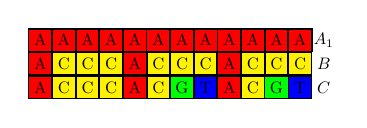
\begin{tikzpicture}[->,>=stealth',shorten >=1pt,auto,node distance=4cm, semithick, scale=0.6, every node/.style={scale=0.6}]   
    \node[draw, fill = red   ] at (0.0, 0  ) {A};
    \node[draw, fill = red   ] at (0.5, 0  ) {A};
    \node[draw, fill = red   ] at (1.0, 0  ) {A};
    \node[draw, fill = red   ] at (1.5, 0  ) {A};
    \node[draw, fill = red   ] at (2.0, 0  ) {A};
    \node[draw, fill = red   ] at (2.5, 0  ) {A};
    \node[draw, fill = red   ] at (3.0, 0  ) {A};
    \node[draw, fill = red   ] at (3.5, 0  ) {A};
    \node[draw, fill = red   ] at (4.0, 0  ) {A};
    \node[draw, fill = red   ] at (4.5, 0  ) {A};
    \node[draw, fill = red   ] at (5.0, 0  ) {A};
    \node[draw, fill = red   ] at (5.5, 0  ) {A};
    \node[                   ] at (6.0, 0  ) {$A_1$};

    \node[draw, fill = red   ] at (0.0, -0.5) {A};
    \node[draw, fill = yellow] at (0.5, -0.5) {C};
    \node[draw, fill = yellow] at (1.0, -0.5) {C};
    \node[draw, fill = yellow] at (1.5, -0.5) {C};
    \node[draw, fill = red   ] at (2.0, -0.5) {A};
    \node[draw, fill = yellow] at (2.5, -0.5) {C};
    \node[draw, fill = yellow] at (3.0, -0.5) {C};
    \node[draw, fill = yellow] at (3.5, -0.5) {C};
    \node[draw, fill = red   ] at (4.0, -0.5) {A};
    \node[draw, fill = yellow] at (4.5, -0.5) {C};
    \node[draw, fill = yellow] at (5.0, -0.5) {C};
    \node[draw, fill = yellow] at (5.5, -0.5) {C};
    \node[                   ] at (6.0, -0.5) {$B$};

    \node[draw, fill = red] at (0.0, -1.0) {A};
    \node[draw, fill = yellow] at (0.5, -1.0) {C};
    \node[draw, fill = yellow] at (1.0, -1.0) {C};
    \node[draw, fill = yellow] at (1.5, -1.0) {C};
    \node[draw, fill = red   ] at (2.0, -1.0) {A};
    \node[draw, fill = yellow] at (2.5, -1.0) {C};
    \node[draw, fill = green ] at (3.0, -1.0) {G};
    \node[draw, fill = blue  ] at (3.5, -1.0) {T};
    \node[draw, fill = red   ] at (4.0, -1.0) {A};
    \node[draw, fill = yellow] at (4.5, -1.0) {C};
    \node[draw, fill = green ] at (5.0, -1.0) {G};
    \node[draw, fill = blue  ] at (5.5, -1.0) {T};
    \node[                   ] at (6.0, -1.0) {$C$};

  \end{tikzpicture}
}

\newcommand{\CreateBdMarkovChain}{
  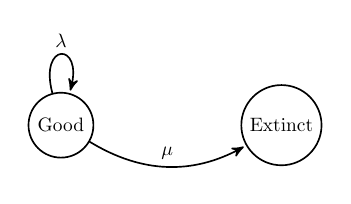
\begin{tikzpicture}[->,>=stealth',shorten >=1pt,auto,node distance=4cm, semithick, scale=0.7, every node/.style={scale=0.7}]   
  \tikzstyle{every state}=[]
  \node[state] (B)              {Good};   
  \node[state] (C) [right of=B] {Extinct};   
  \path (B) edge [loop above] node {$\lambda$} (B)
        (B) edge [bend right] node {$\mu$} (C); 
  \end{tikzpicture}
}

\newcommand{\CreateIncipientSpeciesTree}{
  \begin{tikzpicture}[>=stealth',shorten >=1pt,auto,node distance=4cm, semithick, scale=0.4, every node/.style={scale=0.4}]   
    \tikzstyle{every state}=[]
    % Drawing of the phylogeny
    \begin{scope}[shift={(0,-3)}] 
      \draw (0, 0) -- (2,  0); % stem 
      \draw (2, 0) -- (8,  3) node[anchor=west] {$A_1$};
      \draw[dotted] (4,  -1) -- (5, -0.5); \draw (5, -0.5) -- (8, 1) node[anchor=west] {$B$};
      \draw[dotted] (6,  -2) -- (7, -1.5); \draw (7, -1.5) -- (8, -1) node[anchor=west] {$C$};
      \draw[dotted] (2,0) -- (8, -3) node[anchor=west] {$A_2$};
    \end{scope} % Drawing of the phylogeny
  \end{tikzpicture}
}

\newcommand{\CreatePbdMarkovChain}{
  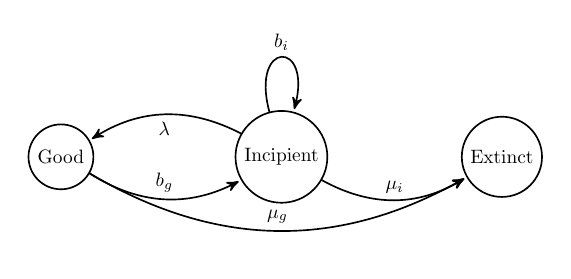
\begin{tikzpicture}[->,>=stealth',shorten >=1pt,auto, node distance=4cm, semithick, scale=0.7, every node/.style={scale=0.7}]   
  \tikzstyle{every state}=[]
  \node[state] (A)              {Good};   
  \node[state] (B) [right of=A] {Incipient};   
  \node[state] (C) [right of=B] {Extinct};   
  \path (A) edge [bend right] node {$b_g$} (B)
        (A) edge [bend right] node {$\mu_g$} (C)
        (B) edge [loop above] node {$b_i$} (B)
        (B) edge [bend right] node {$\lambda$} (A)
        (B) edge [bend right] node {$\mu_i$} (C); 
  \end{tikzpicture}
}


\newcommand{\CreatePosteriorPhylogeny}{
  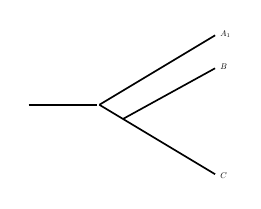
\begin{tikzpicture}[>=stealth',shorten >=1pt,auto,node distance=4cm, semithick, scale=0.3, every node/.style={scale=0.3}]   
    \draw (0, 0) -- (3,  0);
    \draw (3, 0) -- (8, 3) node[anchor=west] {$A_1$};
    \draw (4,-0.6) -- (8, 1.6) node[anchor=west] {$B$};
    \draw (3, 0) -- (8,-3) node[anchor=west] {$C$};

  \end{tikzpicture}
}


\AtBeginSection[]
{
  \begin{frame}
    \frametitle{Table of Contents}
    \tableofcontents[currentsection]
  \end{frame}
}

\titlegraphic{

  \href{http://github.com/richelbilderbeek/Science}{http://github.com/richelbilderbeek/Science}

  
\includegraphics[width=\textwidth,width=.18\textwidth]{rug_logo_big.png}
  \hspace*{0.05in}
  
\includegraphics[width=\textwidth,width=.50\textwidth]{gelifes-header-690x220.png}
  \hspace*{0.05in}
  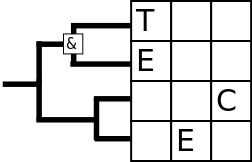
\includegraphics[width=\textwidth,width=.25\textwidth]{tece_logo_2.png}  
}

%%%%%%%%%%%%%%%%%%%%%%%%%%%%%%%%%%%%%%%%%%%%%%%%%%%%%%%%%%%%%%%%%%%%%%%%%%%%%%%%
% References
%%%%%%%%%%%%%%%%%%%%%%%%%%%%%%%%%%%%%%%%%%%%%%%%%%%%%%%%%%%%%%%%%%%%%%%%%%%%%%%%
% Don't. Add references as footnotes instead...
%%%%%%%%%%%%%%%%%%%%%%%%%%%%%%%%%%%%%%%%%%%%%%%%%%%%%%%%%%%%%%%%%%%%%%%%%%%%%%%%
\begin{document}

\frame{\titlepage}

\section[Problem]{Problem}

%%%%%%%%%%%%%%%%%%%%%%%%%%%%%%%%%%%%%%%%%%%%%%%%%%%%%%%%%%%%%%%%%%%%%%%%%%%%%%%%
\begin{frame}
  \frametitle[]{Tree of life\footnotemark}
  \begin{columns}[T]
    \begin{column}{.45\textwidth}
      \begin{block}{}
        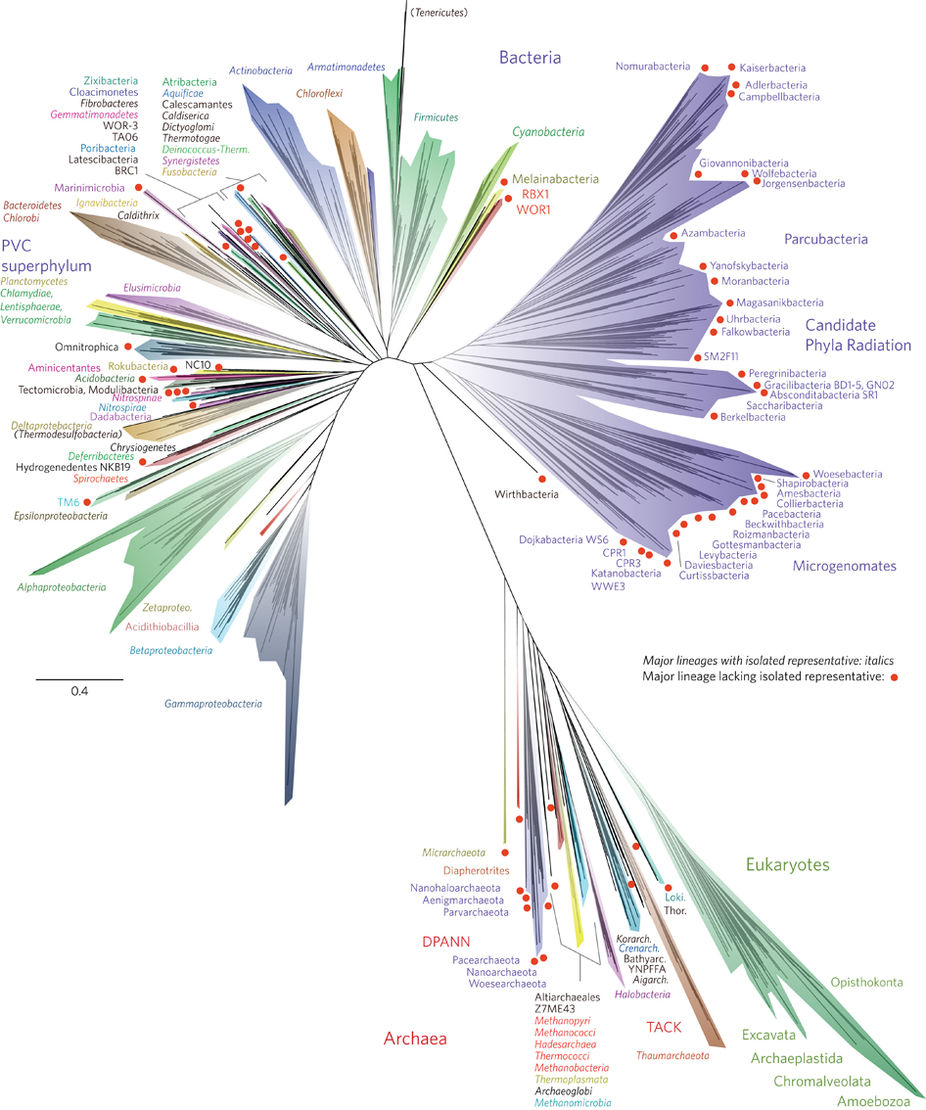
\includegraphics[height=0.65\textheight]{tree_of_life_2016.jpg}
      \end{block}
    \end{column}
    \begin{column}{.5\textwidth}
      \begin{block}{}
        Uses RAxML\footnotemark
      \end{block}
    \end{column}
  \end{columns}
  \footnotetext[1]{Stamatakis, Alexandros. 2014. Bioinformatics 30.9 (2014).}
  % Stamatakis, Alexandros. "RAxML version 8: a tool for phylogenetic analysis and post-analysis of large phylogenies." Bioinformatics 30.9 (2014): 1312-1313.
  \footnotetext[2]{Hug, Laura A., et al. 2016. Nature Microbiology 1 (2016).}
  % Hug, Laura A., et al. "A new view of the tree of life." Nature Microbiology 1 (2016): 16048.
\end{frame}
%%%%%%%%%%%%%%%%%%%%%%%%%%%%%%%%%%%%%%%%%%%%%%%%%%%%%%%%%%%%%%%%%%%%%%%%%%%%%%%%


%%%%%%%%%%%%%%%%%%%%%%%%%%%%%%%%%%%%%%%%%%%%%%%%%%%%%%%%%%%%%%%%%%%%%%%%%%%%%%%%
\begin{frame}
  \frametitle{New giraffe species ... \footnotemark\footnotemark}
  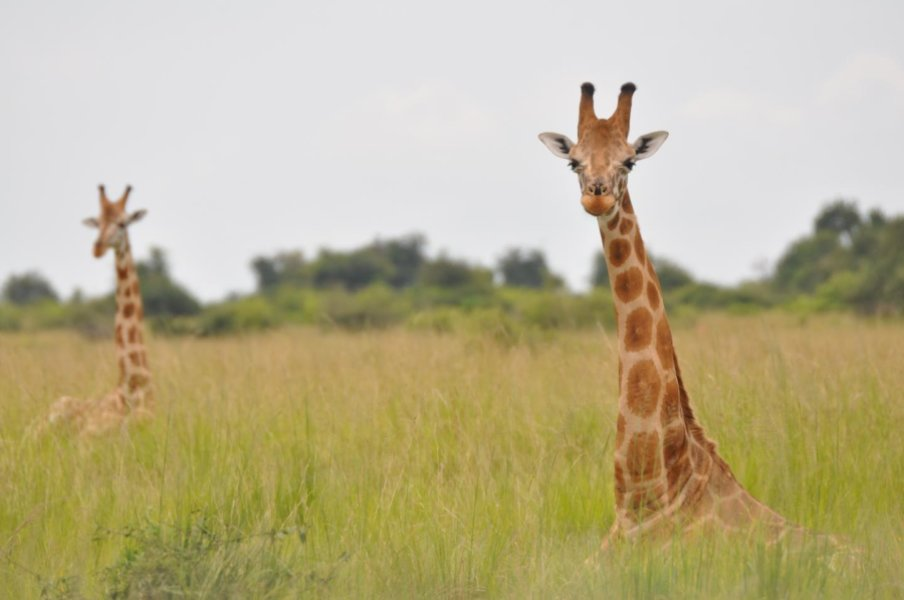
\includegraphics[height=0.8\textheight]{fennessy_2016_nubian_giraffe.jpg}
  \footnotetext[3]{Fennessy, Julian, et al. 2016. Current Biology 26.18.}
  \footnotetext[4]{Picture by Julian Fennessy}
  %\footnotetext[3]{Fennessy, Julian, et al. "Multi-locus analyses reveal four giraffe species instead of one." Current Biology 26.18 (2016): 2543-2549.}
  %\footnotetext[4]{Picture by Julian Fennessy}
\end{frame}
%%%%%%%%%%%%%%%%%%%%%%%%%%%%%%%%%%%%%%%%%%%%%%%%%%%%%%%%%%%%%%%%%%%%%%%%%%%%%%%%

%%%%%%%%%%%%%%%%%%%%%%%%%%%%%%%%%%%%%%%%%%%%%%%%%%%%%%%%%%%%%%%%%%%%%%%%%%%%%%%%
\begin{frame}
  \frametitle{... for quite some time\footnotemark}
  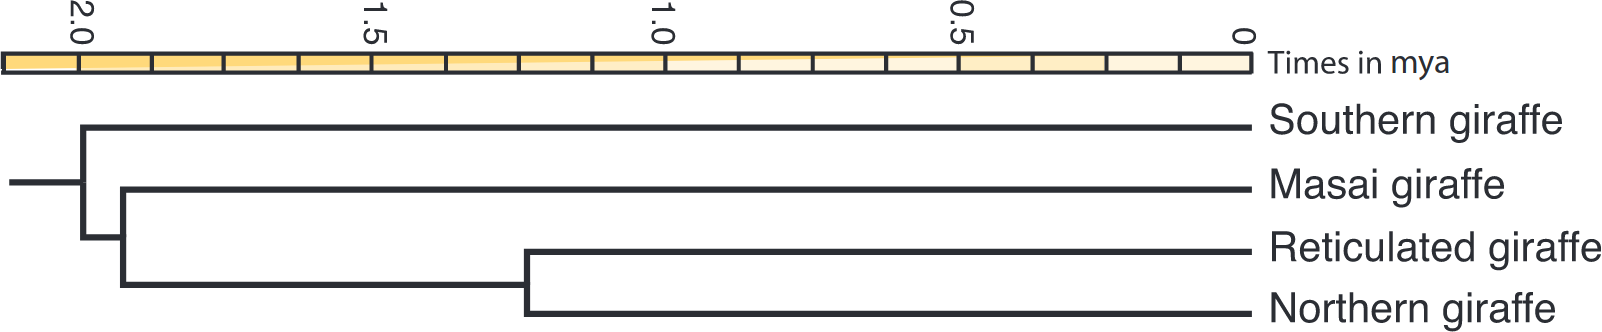
\includegraphics[width=\textwidth]{fennessy_2016_tree.png}
  \footnotetext[5]{Fennessy, Julian, et al. 2016. Current Biology 26.18.}
  % \footnotetext[5]{Fennessy, Julian, et al. "Multi-locus analyses reveal four giraffe species instead of one." Current Biology 26.18 (2016): 2543-2549.}
\end{frame}
%%%%%%%%%%%%%%%%%%%%%%%%%%%%%%%%%%%%%%%%%%%%%%%%%%%%%%%%%%%%%%%%%%%%%%%%%%%%%%%%

\section[Research question]{Research question}

%%%%%%%%%%%%%%%%%%%%%%%%%%%%%%%%%%%%%%%%%%%%%%%%%%%%%%%%%%%%%%%%%%%%%%%%%%%%%%%%
\begin{frame}
  \frametitle{Research question}

  What is the error we make today ...

  \begin{itemize}
    \item in inferring phylogenies
    \item caused by ignoring that speciation takes time to complete?
  \end{itemize}

\end{frame}
%%%%%%%%%%%%%%%%%%%%%%%%%%%%%%%%%%%%%%%%%%%%%%%%%%%%%%%%%%%%%%%%%%%%%%%%%%%%%%%%

\section[Introduction]{Introduction}

%%%%%%%%%%%%%%%%%%%%%%%%%%%%%%%%%%%%%%%%%%%%%%%%%%%%%%%%%%%%%%%%%%%%%%%%%%%%%%%%
\begin{frame}
  \frametitle{Common: from DNA to phylogeny\footnotemark\footnotemark}
  \begin{figure}[]
    \subfloat{
      from \CreateAlignment
      to \CreatePosteriorPhylogeny
      distribution
    }

    \subfloat{
      using 
      
\includegraphics[width=0.15\textwidth]{beast2_logo.png}
      and 
      \CreateBdMarkovChain
    }
  \end{figure}
  \footnotetext[666]{Bouckaert, Remco, et al. 2014. PLoS computational biology 10.4.}
  % Bouckaert, Remco, et al. "BEAST 2: a software platform for Bayesian evolutionary analysis." PLoS computational biology 10.4 (2014): e1003537.
  \footnotetext[666]{Nee, Sean, et al. 1994. Philos Trans R Soc Lond B Biol Sci 344.1309.}
  % Nee, Sean, Robert M. May, and Paul H. Harvey. "The reconstructed evolutionary process." Philosophical Transactions of the Royal Society of London B: Biological Sciences 344.1309 (1994): 305-311.
\end{frame}
%%%%%%%%%%%%%%%%%%%%%%%%%%%%%%%%%%%%%%%%%%%%%%%%%%%%%%%%%%%%%%%%%%%%%%%%%%%%%%%%

%%%%%%%%%%%%%%%%%%%%%%%%%%%%%%%%%%%%%%%%%%%%%%%%%%%%%%%%%%%%%%%%%%%%%%%%%%%%%%%%
\begin{frame}
  \frametitle{Novel: simulating DNA\footnotemark\footnotemark}
  \begin{figure}[]
    \subfloat{
      using
      \CreatePbdMarkovChain
    }

    \subfloat{
      simulate 
      \CreateIncipientSpeciesTree
      and 
      \CreateAlignment
    }

  \end{figure}
  \footnotetext[666]{Etienne, Rampal S., and James Rosindell. 2012. Systematic Biology 61.2.}
  % Etienne, Rampal S., and James Rosindell. "Prolonging the past counteracts the pull of the present: protracted speciation can explain observed slowdowns in diversification." Systematic Biology 61.2 (2012): 204-213.
  \footnotetext[666]{Schliep, Klaus Peter. 2010. Bioinformatics btq706.}
  % Schliep, Klaus Peter. "phangorn: phylogenetic analysis in R." Bioinformatics (2010): btq706.

\end{frame}
%%%%%%%%%%%%%%%%%%%%%%%%%%%%%%%%%%%%%%%%%%%%%%%%%%%%%%%%%%%%%%%%%%%%%%%%%%%%%%%%

%%%%%%%%%%%%%%%%%%%%%%%%%%%%%%%%%%%%%%%%%%%%%%%%%%%%%%%%%%%%%%%%%%%%%%%%%%%%%%%%
\begin{frame}
  \frametitle{Measuring error using nLTT statistic\footnotemark}

  \begin{figure}[]
    \subfloat{
      compare 'true' tree
      \includesvg[width=0.125\textwidth]{example_tree_1}
    }
    \subfloat{
      with inferred tree
      \includesvg[width=0.125\textwidth]{example_tree_2}
    }

    \subfloat{
      using 
      \includesvg[width=0.4\textwidth]{example_nltt_plot}
    }
  \end{figure}

  \footnotetext[666]{Janzen, Thijs et al. 2015. Methods in Ecology and Evolution 6.5.}
  % Janzen, Thijs, Sebastian Höhna, and Rampal S. Etienne. "Approximate Bayesian Computation of diversification rates from molecular phylogenies: introducing a new efficient summary statistic, the nLTT." Methods in Ecology and Evolution 6.5 (2015): 566-575.

\end{frame}
%%%%%%%%%%%%%%%%%%%%%%%%%%%%%%%%%%%%%%%%%%%%%%%%%%%%%%%%%%%%%%%%%%%%%%%%%%%%%%%%

\section[Preliminary results]{Preliminary results}

%%%%%%%%%%%%%%%%%%%%%%%%%%%%%%%%%%%%%%%%%%%%%%%%%%%%%%%%%%%%%%%%%%%%%%%%%%%%%%%%
\begin{frame}
  \frametitle{Longer duration of speciation}

  \begin{figure}[]
    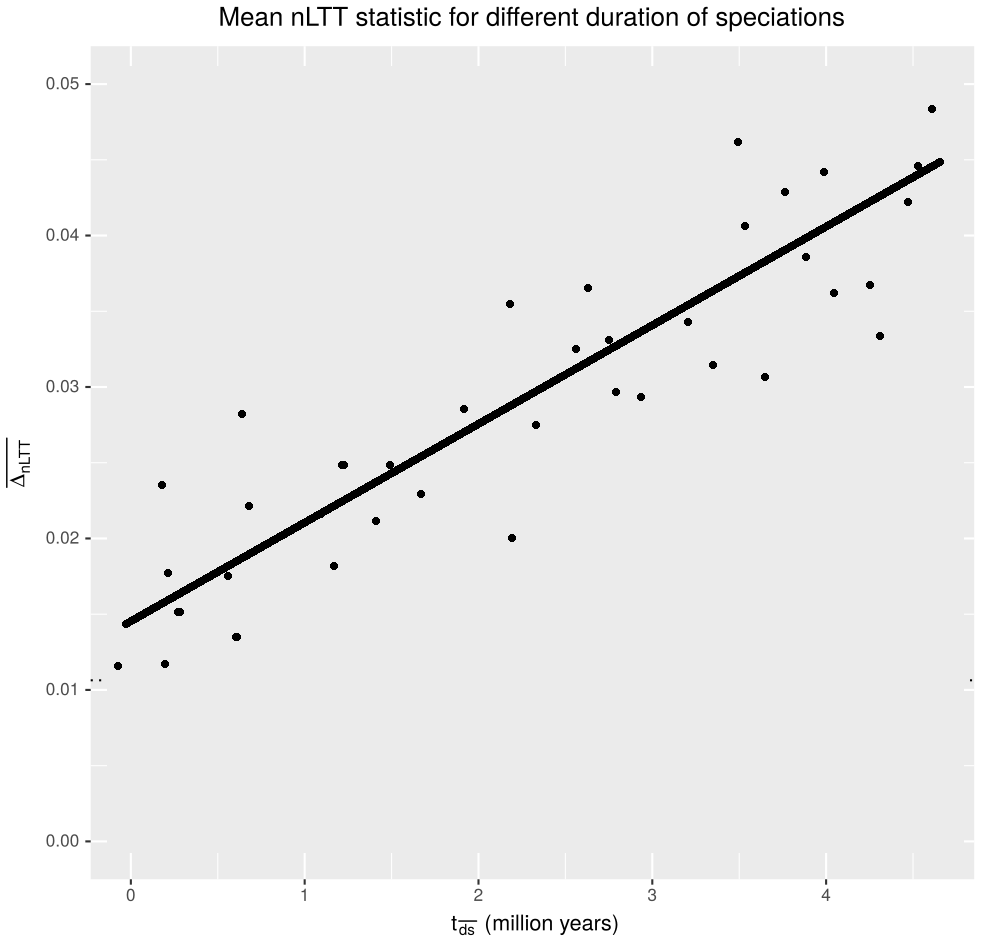
\includegraphics[height=0.8\textheight]{expected_error_mean_durspec.png}
  \end{figure}

\end{frame}
%%%%%%%%%%%%%%%%%%%%%%%%%%%%%%%%%%%%%%%%%%%%%%%%%%%%%%%%%%%%%%%%%%%%%%%%%%%%%%%%

%%%%%%%%%%%%%%%%%%%%%%%%%%%%%%%%%%%%%%%%%%%%%%%%%%%%%%%%%%%%%%%%%%%%%%%%%%%%%%%%
\begin{frame}
  \frametitle{Longer duration of speciation}

  \begin{figure}[]
    \includesvg[height=0.9\textheight]{figure_error_expected_mean_dur_spec_mean}
  \end{figure}

\end{frame}
%%%%%%%%%%%%%%%%%%%%%%%%%%%%%%%%%%%%%%%%%%%%%%%%%%%%%%%%%%%%%%%%%%%%%%%%%%%%%%%%

%%%%%%%%%%%%%%%%%%%%%%%%%%%%%%%%%%%%%%%%%%%%%%%%%%%%%%%%%%%%%%%%%%%%%%%%%%%%%%%%
\begin{frame}
  \frametitle{Effect of bad estimation}

  \begin{figure}[]
    \subfloat{
      \includesvg[width=0.5\textwidth]{figure_error_posterior_nltt_bad_stree}
    }
    \subfloat{
      \includesvg[width=0.5\textwidth]{figure_error_posterior_nltt_bad_post_tree}
    }
  \end{figure}


\end{frame}
%%%%%%%%%%%%%%%%%%%%%%%%%%%%%%%%%%%%%%%%%%%%%%%%%%%%%%%%%%%%%%%%%%%%%%%%%%%%%%%%


%%%%%%%%%%%%%%%%%%%%%%%%%%%%%%%%%%%%%%%%%%%%%%%%%%%%%%%%%%%%%%%%%%%%%%%%%%%%%%%%
\begin{frame}
  \frametitle{Longer DNA alignments}

  \begin{figure}[]
    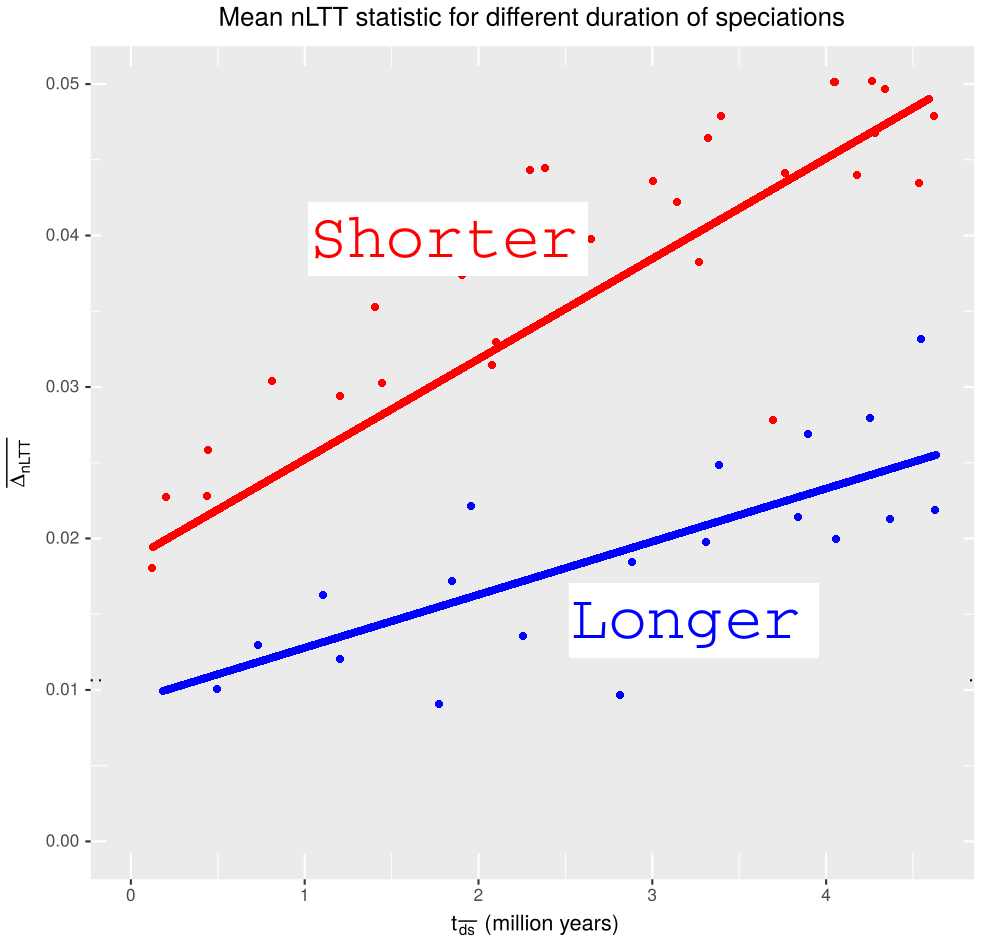
\includegraphics[height=0.8\textheight]{expected_error_mean_durspec_alignment_length.png}
  \end{figure}

\end{frame}
%%%%%%%%%%%%%%%%%%%%%%%%%%%%%%%%%%%%%%%%%%%%%%%%%%%%%%%%%%%%%%%%%%%%%%%%%%%%%%%%

%%%%%%%%%%%%%%%%%%%%%%%%%%%%%%%%%%%%%%%%%%%%%%%%%%%%%%%%%%%%%%%%%%%%%%%%%%%%%%%%
\begin{frame}
  \frametitle{Longer duration of speciation}

  \begin{figure}[]
    \includesvg[height=0.9\textheight]{figure_error_expected_mean_dur_spec_mean_alignment_length}
  \end{figure}

\end{frame}
%%%%%%%%%%%%%%%%%%%%%%%%%%%%%%%%%%%%%%%%%%%%%%%%%%%%%%%%%%%%%%%%%%%%%%%%%%%%%%%%

\section[Preliminary conclusions]{Preliminary conclusions}

%%%%%%%%%%%%%%%%%%%%%%%%%%%%%%%%%%%%%%%%%%%%%%%%%%%%%%%%%%%%%%%%%%%%%%%%%%%%%%%%
\begin{frame}
  \frametitle{Preliminary conclusions}

  It is shown that:
  \begin{enumerate}
    \item $\uparrow$ protractedness leads to $\uparrow$ error
    \item $\downarrow$ DNA sequence leads to $\uparrow$ error
    \item (not shown) sampling subspecies has no effect 
    \item (not shown) number of taxa has no effect
  \end{enumerate}

\end{frame}
%%%%%%%%%%%%%%%%%%%%%%%%%%%%%%%%%%%%%%%%%%%%%%%%%%%%%%%%%%%%%%%%%%%%%%%%%%%%%%%%

%%%%%%%%%%%%%%%%%%%%%%%%%%%%%%%%%%%%%%%%%%%%%%%%%%%%%%%%%%%%%%%%%%%%%%%%%%%%%%%%
\begin{frame}
  \frametitle{if $t \geq 16:00$, then done}
  
  \center
  \Huge
  \faSmileO THANKS! \faSmileO

\end{frame}
%%%%%%%%%%%%%%%%%%%%%%%%%%%%%%%%%%%%%%%%%%%%%%%%%%%%%%%%%%%%%%%%%%%%%%%%%%%%%%%%

\section[Work in progress]{Work in progress}

%%%%%%%%%%%%%%%%%%%%%%%%%%%%%%%%%%%%%%%%%%%%%%%%%%%%%%%%%%%%%%%%%%%%%%%%%%%%%%%%
\begin{frame}
  \frametitle{Current problem}

  Incomplete documentation

\end{frame}
%%%%%%%%%%%%%%%%%%%%%%%%%%%%%%%%%%%%%%%%%%%%%%%%%%%%%%%%%%%%%%%%%%%%%%%%%%%%%%%%


%%%%%%%%%%%%%%%%%%%%%%%%%%%%%%%%%%%%%%%%%%%%%%%%%%%%%%%%%%%%%%%%%%%%%%%%%%%%%%%%
\begin{frame}
  \frametitle{Parameter estimation}

  \begin{figure}[]
    \subfloat{
     given
     \CreatePbdMarkovChain,
    }

    \subfloat{
      then for $\lambda \rightarrow \infty$, becomes 
      \CreateBdMarkovChain
    }

  \itemize{
    \item $\lambda$: speciation rate
    \item $\mu$: extinction rate
  }

  \end{figure}

\end{frame}
%%%%%%%%%%%%%%%%%%%%%%%%%%%%%%%%%%%%%%%%%%%%%%%%%%%%%%%%%%%%%%%%%%%%%%%%%%%%%%%%

%%%%%%%%%%%%%%%%%%%%%%%%%%%%%%%%%%%%%%%%%%%%%%%%%%%%%%%%%%%%%%%%%%%%%%%%%%%%%%%%
\begin{frame}
  \frametitle{Parameter estimation}


  \begin{figure}
    \subfloat{
      
\includegraphics[width=0.15\textwidth]{beast2_logo.png} 
      takes a 
      \CreateAlignment
      and creates
    }

    \subfloat{
      a distribution of $\left\{\mathcal{T}, \hat{\lambda}, \hat{\mu}, \hat{t_0}, \right\}$
    }
    \itemize{
      \item $\mathcal{T}$: a phylogeny
      \item $\hat{\lambda}$: estimated speciation rate
      \item $\hat{\mu}$: estimated extinction rate
      \item $\hat{t_0}$: estimated crown age
    }
  \end{figure}


\end{frame}
%%%%%%%%%%%%%%%%%%%%%%%%%%%%%%%%%%%%%%%%%%%%%%%%%%%%%%%%%%%%%%%%%%%%%%%%%%%%%%%%






%%%%%%%%%%%%%%%%%%%%%%%%%%%%%%%%%%%%%%%%%%%%%%%%%%%%%%%%%%%%%%%%%%%%%%%%%%%%%%%%
\begin{frame}
  \frametitle{Naive expectation}

  \begin{table}
    \centering

    %                           rng_seed sirg siri   scr erg eri age mutation_rate n_alignments
    % article_0_3_2_0_0_549.RDa      549  0.3  0.3 1e+06 0.2 0.2  15          0.05            2
    %                           sequence_length nspp n_beast_runs
    % article_0_3_2_0_0_549.RDa            1000 1000            2
    \subfloat[Parameters to create phylogenies]{
      \begin{tabular}{ | l | l | l | }
        \hline
        $\lambda$ & speciation rate & 0.3 \\
        \hline
        $\mu$ & extinction rate & 0.2 \\
        \hline
        $t_0$ & crown age & 15 \\
        \hline
      \end{tabular}

    }

    \subfloat[Expected parameter estimates]{
      \begin{tabular}{ | l | l | l | l | l | }
        \hline
        $\hat{\lambda}$ & estimated speciation rate & 0.31 & 0.29 & 0.28 \\
        \hline
        $\hat{\mu}$ & estimated extinction rate & 0.19 & 0.21 & 0.2 \\
        \hline
        $\hat{t_0}$ & estimated crown age & 14.9 & 15.1 & 15.2 \\
        \hline
      \end{tabular}

    }
  \end{table}




% article_0_3_2_0_0_549
%    BirthDeath birthRate2 relativeDeathRate2 TreeHeight
% 626   189.5141   18.59102          0.6949177  0.1514966
% 112   191.1941   23.74016          0.3816950  0.1471925
% 709   192.2802   16.17563          0.6062069  0.1457897
% 162   190.5352   22.77061          0.4911272  0.1503252
% 289   190.0760   24.02033          0.2977736  0.1513978

\end{frame}
%%%%%%%%%%%%%%%%%%%%%%%%%%%%%%%%%%%%%%%%%%%%%%%%%%%%%%%%%%%%%%%%%%%%%%%%%%%%%%%%


%%%%%%%%%%%%%%%%%%%%%%%%%%%%%%%%%%%%%%%%%%%%%%%%%%%%%%%%%%%%%%%%%%%%%%%%%%%%%%%%
\begin{frame}
  \frametitle{Real results}

  \begin{table}
    \centering

    %                           rng_seed sirg siri   scr erg eri age mutation_rate n_alignments
    % article_0_3_2_0_0_549.RDa      549  0.3  0.3 1e+06 0.2 0.2  15          0.05            2
    %                           sequence_length nspp n_beast_runs
    % article_0_3_2_0_0_549.RDa            1000 1000            2
    \subfloat[Parameters to create phylogenies]{
      \begin{tabular}{ | l | l | l | }
        \hline
        $\lambda$ & speciation rate & 0.3 \\
        \hline
        $\mu$ & extinction rate & 0.2 \\
        \hline
        $t_0$ & crown age & 15 \\
        \hline
      \end{tabular}

    }

    % article_0_3_2_0_0_549
    %    BirthDeath birthRate2 relativeDeathRate2 TreeHeight
    % 626   189.5141   18.59102          0.6949177  0.1514966
    % 112   191.1941   23.74016          0.3816950  0.1471925
    % 709   192.2802   16.17563          0.6062069  0.1457897
    % 162   190.5352   22.77061          0.4911272  0.1503252
    % 289   190.0760   24.02033          0.2977736  0.1513978
    \subfloat[Parameter estimates]{

      \begin{tabular}{ | l | l | l | l | l | l | }
        % \hline
        % BirthDeath         & 189.514 & 191.194 & 192.28  & 190.535 & 190.076 \\
        \hline
        birthRate2         & 18.591  & 23.7402 & 16.1756 & 22.7706 & 24.0203 \\
        \hline
        relativeDeathRate2 & 0.69492 & 0.3817  & 0.60621 & 0.49113 & 0.29777 \\
        \hline
        TreeHeight         & 0.1515  & 0.14719 & 0.14579 & 0.15033 & 0.1514  \\
        \hline
      \end{tabular}


    }
  \end{table}

\end{frame}
%%%%%%%%%%%%%%%%%%%%%%%%%%%%%%%%%%%%%%%%%%%%%%%%%%%%%%%%%%%%%%%%%%%%%%%%%%%%%%%%




\end{document}